\documentclass[tikz,border=2mm]{standalone}
\begin{document}
	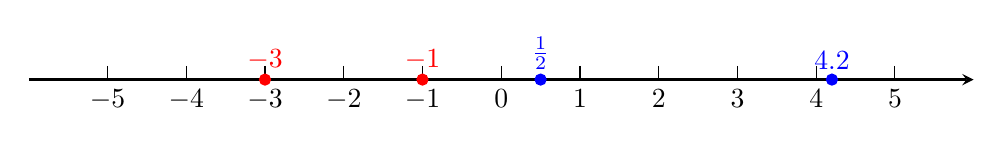
\begin{tikzpicture}
  		\draw [black, thick, ->, >=stealth] (-6,0) -- (6,0); % ->��ͷ��,>=stealth��ʵ�ļ�ͷ
		%\foreach \x in {-9, -8, -7, -6, -5, -4, -3, -2, -1, 0, 1, 2, 3, 4, 5, 6, 7, 8, 9}
		\foreach \x in {-5, ..., 5}
			\draw (\x cm,5pt) -- (\x cm,0pt) node[anchor=north] {$\x$};
		% -3, 4.2, -1, 1/2
		\draw [red, fill=red] (-3, 0) circle(2pt) node [above] {$-3$}; 
		\draw [blue, fill=blue] (4.2, 0) circle(2pt) node [above] {$4.2$}; 
		\draw [red, fill=red] (-1, 0) circle(2pt) node [above] {$-1$}; 
		\draw [blue, fill=blue] (1/2, 0) circle(2pt) node [above] {$\frac{1}{2}$}; 		
	\end{tikzpicture}    
\end{document}
